\section{Rust Embedded Library}
\label{sec:rust_embedded_library}

When we consider {\std}'s dependencies, shown in \autoref{fig:rust:librust}, we see that the crate is not suitable for a bare-metal application because it depends on an \gls{os} to be present.
The dependency on either a Unix or a Windows \gls{os} excludes {\std} and all of its dependents from being used directly with the EFM32.
This section presents some of the libraries provided by {\rust} that can be used in a bare-metal system, and how and why they are composed into what we refer to as the \gls{rel}.

\begin{figure}[H]
  \begin{center}
    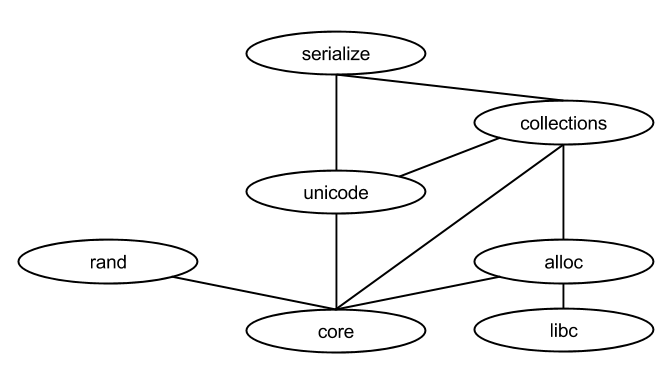
\includegraphics[scale=0.3]{figures/background/rust/embedded-rust-lib.png}
  \end{center}
  \caption{\rust Embedded Library}
  \label{fig:rust:rel}
\end{figure}

\subsection{Allocation}
\label{sec:rust:allocation}

The \gls{rcl} does not use or expose any heap allocation.
Heap allocation is introduced through the \code{Box} type defined in the allocation library.

\subsection{The Collection Library}

The {\rust} collection library provides the data structures shown in \autoref{tab:rust:collections}.

\begin{table}[H]
  \begin{tabular}{l}
    Binary Heap \\
    Binary Tree Map \\
    Binary Tree Set \\
    Bit Set \\
    Bit Vector \\
    Enum Set \\
    Linked List \\
    Vector \\
    Vector Dequeue \\
    Vector Map \\
    String \\
  \end{tabular}
  \caption{\rust Collection Library}
  \label{tab:rust:collections}
\end{table}

We look at some of the data structures in this section.

\subsubsection{Vector}

The Vector is an important data structure both in direct usage but also as a building block for other data structures.
In essence it is a growable heap allocated list of values of the same type.

\subsubsection{String}

In \autoref{par:rust:str} we discussed the \concept{string slice}.
The \code{String} defined in the collection library is a heap allocated mutable string.

\subsection{libc}

The heap allocation library described in \autoref{sec:rust:allocation} depends on the \lib{libc} crate abstraction.
The \lib{libc} library provided in the standard library provides bindings for the {\C} standard library and platform specific libraries.
\gls{rel} depends on \lib{libc} for the low level memory operations \func{malloc}, \func{realloc} and \func{free}.
The details of this implementation is found in \autoref{sec:impl:libc}. \todo{Update reference to implementation chapter part about libc implementation}

\subsection{Notable missing functionality in REL}

- Reference Counted GC
